\documentclass[a4paper,12pt]{article}
\usepackage[utf8]{inputenc}
\usepackage[polish]{babel}
\let\lll\undefined % do babelu, avoiding conflict
\usepackage{polski}
\selectlanguage{polish}
\usepackage[T1]{fontenc}
\frenchspacing
\usepackage{indentfirst}
\usepackage{multicol} %https://www.sharelatex.com/learn/Multiple_columns
\usepackage{float} % option locking floats: [H]


\usepackage{amssymb}
\usepackage{amsmath}
\usepackage{amsfonts}
 
\usepackage[pdftex,dvipsnames]{xcolor} %red, green, blue, yellow, cyan, magenta, black, white
%polskie tabelki
\usepackage[nottoc]{tocbibind}

% Kropki w liczebnikach porzadkowych
\usepackage{titlesec}
\titlelabel{\thetitle.\quad}


\setlength{\parskip}{0.3\baselineskip}%
% \setlength{\parindent}{0pt}%

%polskie przypisy
\usepackage{caption}
\captionsetup{labelsep=period}
\captionsetup{font=small,labelfont=bf,labelsep=period,justification=centering}
\addto\captionspolish{\renewcommand{\figurename}{Rys.}}
\addto\captionspolish{\renewcommand{\tablename}{Tab.}}
\addto\captionspolish{\renewcommand{\seename}{zob.}}

\usepackage{geometry}
 \geometry{
 a4paper,
 %total={170mm,247mm}, % 170 257 20 20
 left=20mm,
 right=20mm,
 top=20mm,
 bottom=25mm,
 }   
   


\usepackage{listings}
\definecolor{mygreen}{RGB}{28,172,0} % color values Red, Green, Blue
\definecolor{mylilas}{RGB}{170,55,241}
% \newcounter{listing}
% \newenvironment{listing}[1][]{
% \refstepcounter{listing}\par\medskip \textbf{Kod~\thelisting. #1} \rmfamily}{\medskip}

\lstset{language=Matlab,%
    %basicstyle=\color{red},
    breaklines=true,%
    morekeywords={matlab2tikz},
    keywordstyle=\color{blue},%
    morekeywords=[2]{1}, keywordstyle=[2]{\color{black}},
    identifierstyle=\color{black},%
    stringstyle=\color{mylilas},
    commentstyle=\color{mygreen},%
    showstringspaces=false,%without this there will be a symbol in the places where there is a space
    numbers=left,%
    numberstyle={\tiny \color{black}},% size of the numbers
    numbersep=9pt, % this defines how far the numbers are from the text
    emph=[1]{for,end,break},emphstyle=[1]\color{red}, %some words to emphasise
    %emph=[2]{word1,word2}, emphstyle=[2]{style},    
    basicstyle=\small\ttfamily,
    frame=single,
    float
}


% \usepackage{svg}
%SVG for the first time using inkscape: for i in *.svg; do inkscape -D -z --file=$i  --export-pdf="${i%.*}.pdf" --export-latex .; done




\usepackage{xargs}                      % Use more than one optional parameter in a new commands
%
\usepackage[colorinlistoftodos,prependcaption,textsize=tiny]{todonotes}
\newcommandx{\unsure}[2][1=]{\todo[linecolor=red,backgroundcolor=red!25,bordercolor=red,#1]{#2}}
\newcommandx{\change}[2][1=]{\todo[linecolor=blue,backgroundcolor=blue!25,bordercolor=blue,#1]{#2}}
% \newcommandx{\info}[2][1=]{\todo[linecolor=OliveGreen,backgroundcolor=OliveGreen!25,bordercolor=OliveGreen,#1]{#2}}
% \newcommandx{\improvement}[2][1=]{\todo[linecolor=Plum,backgroundcolor=Plum!25,bordercolor=Plum,#1]{#2}}
% \newcommandx{\thiswillnotshow}[2][1=]{\todo[disable,#1]{#2}}

% \missingfigure[figwidth=6cm]{Testing a long text string}


\usepackage[section]{placeins} %\FloatBarrier
% \usepackage{hyperref}
   
\usepackage{fancyhdr}
\setlength{\headheight}{38pt}
\pagestyle{fancy}

\lhead{Sprawozdanie z grantu rektorskiego koła SKIK 2017}     \rhead{\today\quad
\includegraphics[width=1.5cm]{logo_skik}}
\lfoot{}            \cfoot{}        \rfoot{strona \thepage/7}

\title{Projekt przedmiotu Sieci Neuronowe i Neurokomputery wydziału EiTI Politechniki Warszawskiej}
\author{Artur Dobrogowski}


%\font\radikalwut=radikalwut at 36pt
\newcommand{\radikalwut}{}

\begin{document}

%
\begin{titlepage}
    \centering
    {\scshape\Large {\radikalwut Politechnika Warszawska}\\\par Wydział Elektroniki i Technik Informacyjnych\\Instytut Radioelektroniki i Technik Multimedialnych \par}
    \vspace{1cm}
    {\huge\scshape\bfseries Sprawozdanie\\\par}
    {\scshape\Large z pracy naukowo-badawczej własnej\\ finansowanej z grantu rektorskiego za rok 2017\\\par}
%     {\Large Umowa numer XXX Y/????/????\\\par}
    \vspace{1cm}
    {\Large\bfseries Budowa mobilnej stacji naziemnej do odbioru danych APRS z balonów stratosferycznych\\\par}
    \vspace{1cm}
    {\Large\textsl {Studenckie Koło Inżynierii Kosmicznej}\par}
    \vfill
    Wykonawcy: \par
    {\small
    \begin{multicols}{2}

    \par Artur \textsc{Dobrogowski} 
    \par Michał \textsc{Kocon}
    \par Maciej \textsc{Trębiński}
    \par Krzysztof \textsc{Wasilewski}
    \end{multicols}
}
    Kierownik pracy:\par
    dr inż. Krzysztof \textsc{Kurek}

    \vfill

% Bottom of the page
    {\large \today\par}
\end{titlepage}

\tableofcontents

\section{Wprowadzenie}


Balon stratosferyczny pozwala na wyniesienia podczepionego pod nim ładunku na wysokość około 35 km nad poziom morza, na której panuje niskie ciśnienie i niska temperatura, czyli warunki zbliżone do środowiska przestrzeni kosmicznej. Stratosferyczne misje balonowe mogą być więc tanim sposobem na testowanie poprawnego działania układów zbudowanych przez studentów, a przewidzianych do pracy w przestrzeni kosmicznej. Jednocześnie umieszczenie różnych czujników w gondoli przyczepionej do balonu pozwala na pomiary różnych parametrów w atmosferze, w funkcji wysokości nad poziomem terenu. Misje takie są coraz częściej organizowane w Polsce, zarówno przez studentów np. ze Studenckiego Koła Astronautycznego PW, jak  również przez różne stowarzyszenia zrzeszające entuzjastów balonów i radioamatorów. Również SKIK, w swojej dotychczasowej działalności zrealizował kilka misji balonowych.

Kluczowym elementem misji balonowej jest przesył informacji na ziemię łączem radiowym, do czego jest potrzebna mobilna naziemna stacja odbiorcza, aby mieć możliwość odbioru danych przesyłanych niezależnie od miejsca startu misji. Ze względu na jakość odbioru, ważne jest aby stacja była z dala od źródeł zakłóceń i w pobliżu miejsca startu. W związku z tym istnieje potrzeba konstrukcji takiej stacji. Stacja mogłaby być wykorzystywana do odbioru transmisji, takich jak komunikatów z balonów meteorologicznych jak również w przyszłych misjach balonowych Studenckiego Koła Inżynierii Kosmicznej.

\section{Cel projektu}

Celem projektu jest opracowanie mobilnej stacji do łączności radiowej z balonem ze szczególnym zwróceniem uwagi na pasma radioamatorskie. Stacja składa się z:
\begin{itemize}
    \item statywu z elektronicznie sterowanymi antenami przy pomocy silników krokowych umożliwiających zmianę orientacji anten w płaszczyźnie azymutu i elewacji,
    \item wzmacniacza sygnału przychodzącego z anteny,
    \item zestawu filtrów pasmowo przepustowych,
    \item radia programowalnego (SDR – Software Defined Radio) do przetworzenia sygnału (wykorzystane zostało radio będące na stanie Laboratorium Technologii Kosmicznych WEiTI), do którego stworzone zostało oprogramowanie umożliwiające odbiór sygnałów
\end{itemize}  

	Opracowana stacja pozwala na odbiór sygnałów w paśmie radioamatorskim: UHF 430 MHz (opcjonalnie w paśmie VHF 140 MHz). 
	Stworzone oprogramowanie do radia programowalnego SDR umożliwia odbiór pakietów APRS – automatycznego systemu powiadamiania o pozycji, który jest zwykle wykorzystywany do lokalizacji balonów w misjach. Wykorzystanie radia programowalnego SDR pozwoli w przyszłości na proste dostosowanie stacji do odbioru innych typów sygnałów (które mogą być przesyłane z balonu) tylko przez zmiany oprogramowania, bez konieczności zmian sprzętowych (jeśli transmisja będzie realizowana w obsługiwanym paśmie częstotliwości).

	Wynikiem prac jest między innymi oprogramowanie pozwalające na odbiór danych systemu APRS i danych podczas trwania misji, z wykorzystaniem radia programowalnego SDR.
	Gotowa stacja stanowi atrakcyjny obiekt zainteresowania do zaprezentowania np. w trakcie targów studenckich kół naukowych KONIK, co pomoże w popularyzacji tematyki związanej z systemami satelitarnymi.
	Wiedza i doświadczenie inżynierskie  zdobyte przez członków Koła w trakcie realizacji projektu pozwolą myśleć o wzięciu udziału w edukacyjnych projektach balonowych organizowanych pod patronatem Europejskiej Agencji Kosmicznej.

\section{Koncepcja mobilnej stacji naziemnej}

Zgodnie z planem projektu powstała stacja składająca się z:

\begin{itemize}
 \item dwu-częściowego rotora wraz ze sterownikiem, czujnikami położenia i kompasem,
 \item wykorzystanego radia programowalnego SDR z oprogramowaniem do dekodowania odbieranego sygnału,
 \item układu FPGA z możliwością realizacji własnego demodulatora na innym paśmie,
 \item układu zasilania składającego się z: 
    \begin{itemize}
    \item akumulatora samochodowego o pojemności 20Ah i napięciu 12 V,
    \item przetwornicy do napięcia 5V do zasilenia układów logicznych rotora,
    \item prostownikia do ładowania akumulatora,
    \item przetwornicy do napięcia zmiennego 230V ze standardowym gniazdkiem do zasilania ewentualnych peryferiów takich jak laptop,
    \end{itemize}
\end{itemize}

Ponieważ nie mamy wykształcenia w zakresie wykonywania konstrukcji mechanicznych to nasz projekt jest realizacją wysoce amatorską, ale funkcjonalną. Największym wyzwaniem był dobór odpowiednich przekładni do uzyskania precyzyjnych (wolnych) obrotów i dużego momentu siły.

Schemat ideowy działania całej stacji przedstawiono na rysunku \ref{stacschem}.

\begin{figure}[!htbp]
    \centering
    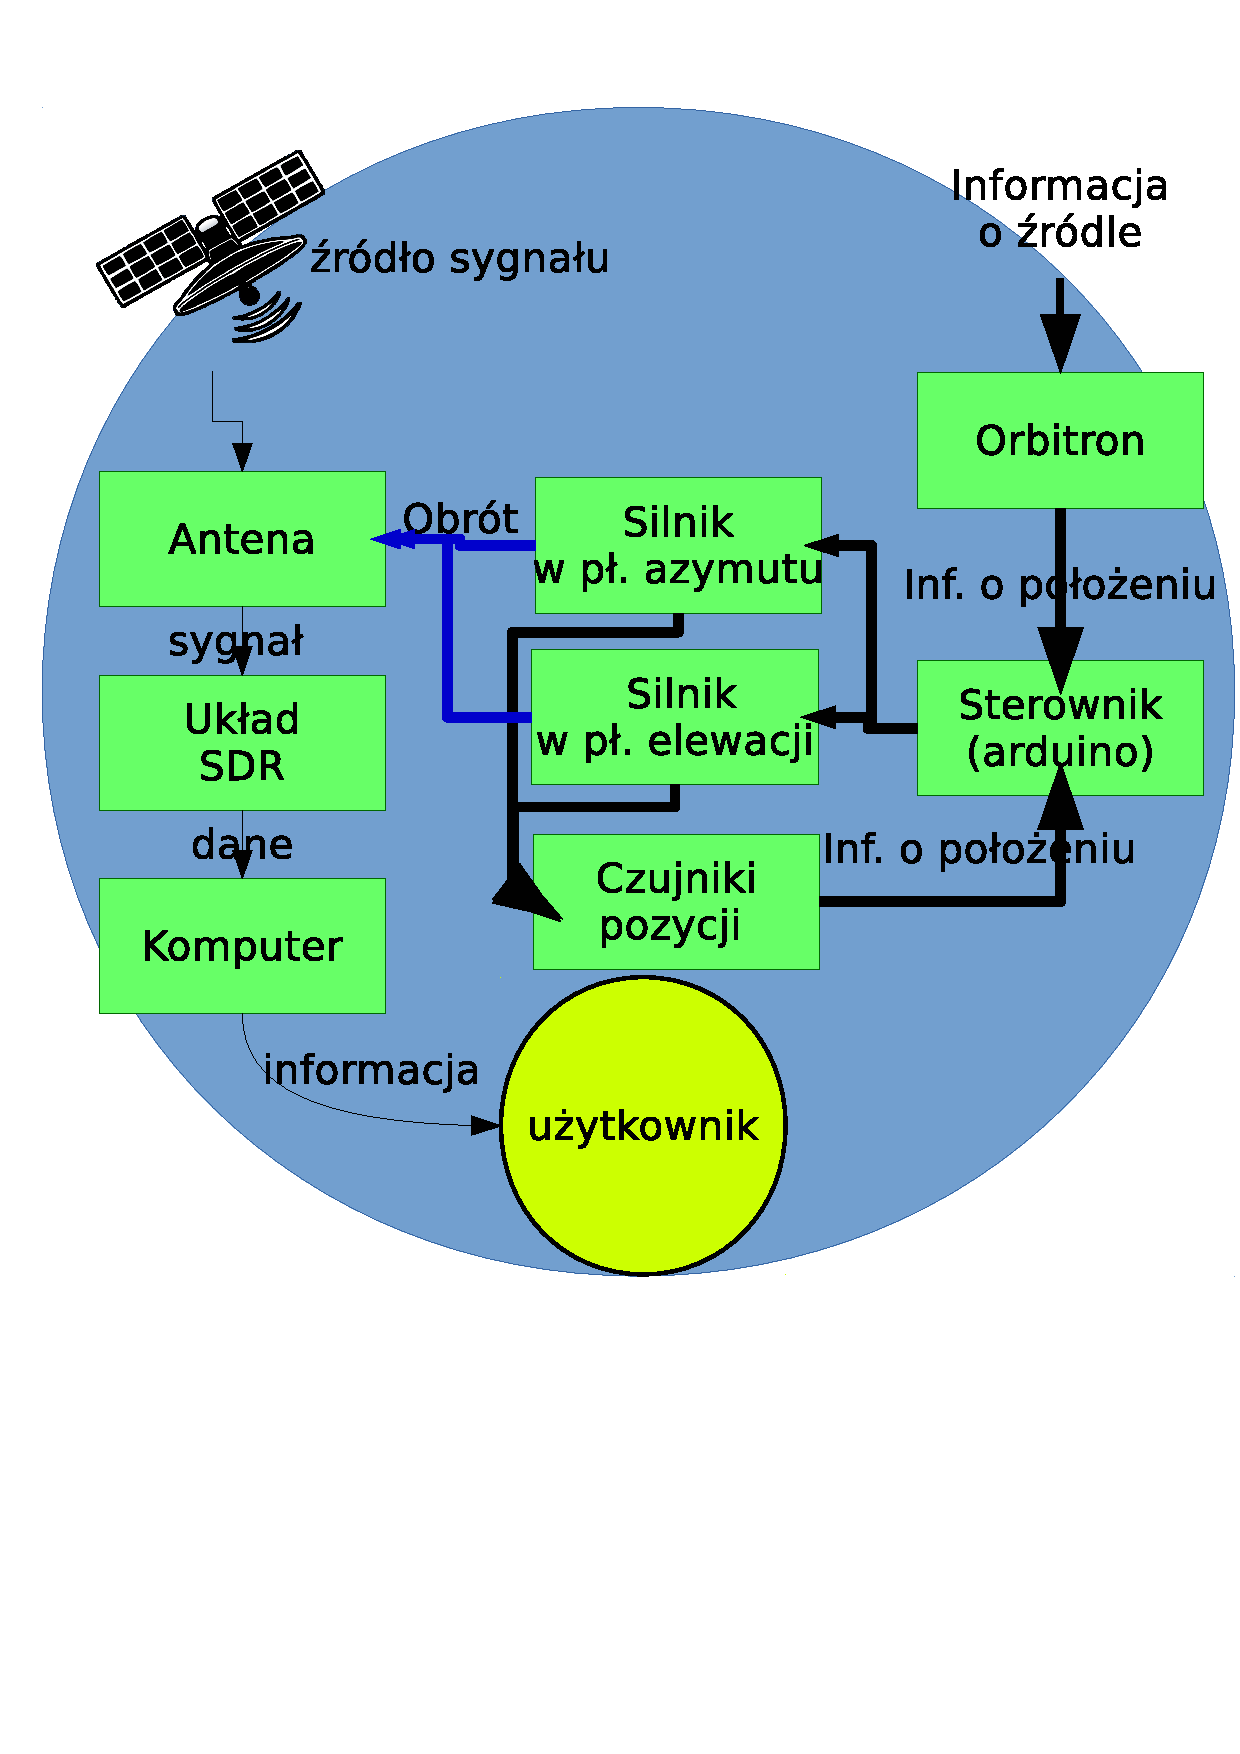
\includegraphics[width=0.7\textwidth]{schemat_skik2017}
    \caption{Schemat blokowy systemu stacji naziemnej}
    \label{stacschem}
\end{figure}

\section{Rotor do sterowania antenami w płaszczyźnie azymutu i elewacji}

Rotor był zaprojektowany i stworzony przez nas od podstaw. 

\section{Sterowanie}

Do sterowania rotorem wykorzystano możliwości programu Orbitron, który pozwala śledzić ruch satelit poruszających się na orbicie okołoziemskiej. Użytkownik jest w stanie otrzymać informacje o położeniu danego satelity na orbicie oraz wysyłać komunikaty z informacją o kącie azymutu i elewacji anteny jaki należy ustawić, żeby namierzyć wybranego satelitę. Na Rys. \ref{fig:rotor} poniżej zamieszczono widok ekranu głównego aplikacji. 

\begin{figure}[h]
	\centering
		\includegraphics[width=0.7 \textwidth]{orbitron}
	\caption{Widok ekranu głównego programu Orbitron}	
	\label{fig:rotor}
\end{figure}

Aby nawiązać komunikację z układem sterującym rotorami zainstalowano aplikację, będącą dodatkiem do programu Orbitron - \textit{DDE Orbitron To Serial} \cite{dde}. Program na bieżąco może pobierać informacje o położeniu satelit i wysyłajać komunikaty poprzez port szeregowy do układu sterującego rotorem.


\begin{figure}[h]
	\centering
		\includegraphics[width=0.7 \textwidth]{DDEOrbitronToSerialScreenShot}
	\caption{Widok okienka aplikacji DDE Orbitron To Serial}	
	\label{fig:rotor}
\end{figure}

Komunikaty z informacją o kącie elewacji i azymutu anteny są wysyłane bezpośrednio do płytki Arduino Uno. Program mikrokontrolera umożliwia sterowanie dwoma silnikami rotora oraz jako sprzężenie zwrotne odbiera dane z enkoderów umieszczonych na osiach silników. Mikrokontroler zlicza impulsy odebrane z czujników co daje pełną informację o rzeczywistym ustawieniu anteny i umożliwia ewentualną korektę. Silniki rotora są silnikami prądu stałego z przekładnią i pozwalają na obrót ze stałą prędkością, więc aby obrócić oś o określony kąt zbadano jaka ilość impulsów enkodera odpowiada pełnemu obrotowi. 

\section{Część radiowa}
\subsection{Automatic Position Reporting System (APRS)}
% Do wykonania przetwarzania w części radiowej wykorzystaliśmy radio
System APRS jest systemem radiowym służącym do przesyłu krótkich wiadomości w radioamatorskim paśmie UKF. Jednym z zastosowań jest przesył danych meteorologicznych czy pozycyjnych z modułu GPS.

Transmisja odbywa się w trybie bezpołączeniowym, a wiadomość może być odebrana przez wiele stacji. APRS w Europie pracuje na częstotliwości 144,8MHz. Przepływność 1200 baud/s przy dwuwartościowej modulacji AFSK zapewnia możliwość przesyłu jedynie podstawowych informacji jednocześnie zajmując wąskie pasmo mieszczące się w zakresie słyszalnym. Ta właściwość umożliwia dekodowanie sygnału APRS za pomocą karty dźwiękowej komputera. 

System APRS bazuje na cyfrowej technice krótkofalarskiej PacketRadio. Bazuje ona na protokole AX.25. Struktura ramkowa bazuje na ramce UI protokołu AX.25. Została ona zaprezentowana w tabeli \ref{ax25}.

\begin{table}
\centering
\begin{tabular*}{\textwidth}{|p{1.2cm}|p{0.8cm}|p{1.65cm}|p{1.2cm}|p{1cm}|p{1.5cm}|p{2.1cm}|p{2cm}|p{0.7cm}|p{0.7cm}|}
\hline
 & Flaga & Adres przeznaczenia (adresat) & Adres źródła (nadawca) & Adres digi (ścieżka) & Pole kontrolne (UI) & Identyfikacja protokołu & Pole informacji & FCS & Flaga\\\hline
Liczba bajtów & 1 & 7 & 7 & 0-56 & 1 & 1 & 1-256 & 2 & n \\\hline
\end{tabular*}
\caption{Struktura ramki protokołu AX.25}
\label{ax25}
\end{table}

% Radio które posiadaliśmy w laboratorium USRP-2932 niestety nie nadaje się do odbioru sygnału APRS ze względu na dolną granicę pasma 400 MHz. Zamiast tego wykorzystaliśmy je do odbioru transmisji o modulacji LoRa wykorzystując jako nadajnik układ z poprzedniego projektu: Orange Pi połączony z układem nadawczym. Do testów transmisji APRS wykorzystaliśmy inne radio programowalne.
% 

Pole informacji ma następującą strukturę jak w tabeli \ref{str}

\begin{table}
\centering
\begin{tabular}{|l|l|l|l|l|}
\hline
  & Identyfikator danych & Dane & Rozszerzenie danych & Komentarz\\\hline
Liczba bajtów & 1 & n & 7 & n\\\hline
\end{tabular}
\caption{Struktura pola informacji ramki protokołu AX.25}
\label{str}
\end{table}

Radio które posiadaliśmy w laboratorium USRP-2932 niestety nie nadaje się do odbioru sygnału APRS ze względu na dolną granicę pasma 400 MHz. Zostanie ono jednak użyte do odbioru systemu LoRa, wykorzystując jako nadajnik układ z poprzedniego projektu: Orange Pi połączony z układem nadawczym firmy Hoperf. Do odbioru sygnału zostały bloki funkcyjne GNURadio implementujące odbiornik systemu LoRa. Sygnał odbierany przez radio SDR zostaje przekazany na blok LoRa Receiver, który dokonuje demodulacji sygnału
\begin{figure}[!htbp]
 \includegraphics[width=0.8\textwidth]{lora_pic}
 \centering
 \caption{Schemat blokowy GNURadio - odbiornik systemu LoRa.}
\end{figure}


Do odbioru sygnału APRS zostanie wykorzystany odbiornik bazujący na Realtek RTL2832U, pozwalający na bezpośredni przesył strumienia I/Q poprzez złącze USB. Za pomocą sterownika rtl-sdr, sygnał APRS jest traktowany jak źródło dzwięku, które następnie podane na program Xastir pozwala na bezpośredni odbiór wiadomości oraz lokalizację na mapie w czasie rzeczywistym.

\begin{figure}[!htbp]
 \includegraphics[width=\textwidth]{xastir}
 \centering
 \caption{Widok programu Xastir.}
\end{figure}

\subsubsection{Demodulator BFSK}

Dodatkowo w ramach grantu napisano demodulator sygnału BFSK (np. APRS) w języku VHDL do zreazlizowania układzie FPGA z przetwornikiem analogowo-cyfrowym. Dzięki temu możliwe będzie przeniesienie oprogramowania realizującego odbiór sygnału z komputera PC do układu FPGA wewnątrz modułu SDR. 

BFSK \emph{(binary frequency shift keying)} to cyfrowa modulacja wykorzystywana  między innymi w komunikacji APRS (służących do podawania pozycji przez radio). Polega na nadawaniu stałego sygnału sinusuidalnego o częstotliwości F0 dla bitu 0 lub częstotliwości F1 dla bitu 1. Przykładowy przebieg pokazano na rysunku \ref{bfsk}

Na obrazku \ref{fpga} przedstawiono wyniki symulacji demodulatora, a na schemacie \ref{bfsk_demodulator} widać schemat blokowy symulowanego demodulatora.


\begin{figure}[!htbp]
 \includegraphics[width=\textwidth]{bfsk}
 \centering
 \caption{Przebieg sygnału o modulacji BFSK}
 \label{bfsk}
\end{figure}


\begin{figure}[!htbp]
 \includegraphics[width=0.35\textwidth]{bfsk_demodulator}
 \centering
 \caption{Schemat blokowy demodulatora BFSK}
 \label{bfsk_demodulator}
\end{figure}


W symulacji sygnał FSK dostarczany do ADC miał odpowiednio częstotliwości 1200Hz i 2200Hz dla F0 i F1.  Sygnał był spróbkowany z Fs = 48kHz., użyty ADC to MCP3208. FPGA komunikuje się z ADC po szynie SPI. Następnie sygnał FSK trafia do demodulatora zaimplementowanego w FPGA \ref{bfsk_demodulator}.  W demodulatorze ten sygnał jest opóźniony o k próbek, a następnie pomnożony z aktualną próbką. Potem znajduje się filtr dolno przepustowy o częstotliwości granicznej równej połowie bitów na sekundę. Otrzymany sygnał jest zdemodulowany.

Opóźnienie k jest policzone na bazie znalezienia minima poniższego równania.

\begin{equation}
d(k) = |\cos(2\pi F_0 k T_e) - \cos(2\pi F_1 k T_e) |
\end{equation}
Gdzie {$T_e$ - okres próbkowania, $k$ - opóźnienie sygnału}.

\begin{figure}[!htbp]
 \includegraphics[width=\textwidth]{symulacja}
 \centering
 \caption{Wynik symulacji demodulacji APRS na FPGA}
 \label{fpga}
\end{figure}

% Okazało się, że gotowe projekty oprogramowania demodulatora zarówno APRS jak i LoRa są dostępne w internecie z otwartym oprogramowaniem w GNU radio, więc wystarczyło je przetestować w naszych układach.

\section{Podsumowanie i testy stacji}

Testy stacji stanowiły testy części radiowej i konstrukcyjnej. W ramach grantu kupiono balon na misję balonową, aby wraz z układem z poprzedniego grantu przetestować łącze radiowe w praktycznych warunkach.

\subsection{Test współpracy z oprogramowaniem Orbitron}

W celów testu wyznaczyliśmy w programie symulowany przelot stacji ISS w okolicach Warszawy i włączyliśmy nasz sterownik do wodzenia anteną za stacją ISS będącą najszybciej poruszającym się obiektem na bliskiej orbicie.

Oprogramowanie zadziałało poprawnie i stacja była sterowana za pośrednictwem komputera. W tym teście okazało się, że stacja ISS przy bliskim przelocie jest znacząco zbyt szybko poruszającym się obiektem dla naszego rotora. Rotor nadążął za zmianami w płaszczyźnie elewacji, ale zmiany azymutalne były zbyt duże. Jak wcześniej wspomniano, można przyspieszyć obroty zwiększając napięcie, ale ogólnie nie przewidywaliśmy śledzenia tak szybkich obiektów. Na zakończenie kilkunastosekundowego testu zrobiliśmy pomiar zewnętrznym kompasem. Jest to przedstawione na rysunku \ref{kompas}.

Test orientacji w płaszczyźnie azymutu wykazał błąd na poziomie $\pm 3^o$, ze względu na niską dokładność użytego kompasu w module. Z drugiej strony potencjalna rozdzielczość rotora w jednostce na impuls enkodera wynosi $0.02^o$ w płaszczyźnie elewacji i $0.2^o$ w płaszczyźnie azymutu dzięki wolnym obrotom. W związku z tym dodaliśmy opcję ręcznego wprowadzenia kalibracji orientacji z komputera jeśli zajdzie potrzeba uzyskania większej dokładności.

Wykonaliśmy test obrotu dookoła, aby sprawdzić czy sterownik steruje poprawnie i nie zerwie kabla sterownika. Rotor poprawnie zaprogramowany nie zerwał kabla i zaczął obracać się w przeciwnym kierunku (o ujemny kąt) aby wykonać pełen obrót.

\begin{figure}[h]
	\centering
		\includegraphics[width=0.7 \textwidth]{testy/antenaS}
	\caption{Antena wskazuje kierunek południowy}	
	\label{fig:antenaS}
\end{figure}

\begin{figure}[h]
	\centering
		\includegraphics[width=0.7 \textwidth]{testy/pojawia}
	\caption{Satelita ISS pojawia się nad horyzontem}	
	\label{fig:pojawia}
\end{figure}

\begin{figure}[h]
	\centering
		\includegraphics[width=0.7 \textwidth]{testy/pojawia}
	\caption{Satelita ISS pojawia się nad horyzontem}	
	\label{fig:pojawia}
\end{figure}


\begin{figure}[h]
	\centering
		\includegraphics[width=0.7 \textwidth]{testy/zenit}
	\caption{Satelita ISS w zenicie}	
	\label{fig:zenit}
\end{figure}


\begin{figure}[h]
	\centering
		\includegraphics[width=0.7 \textwidth]{testy/znika}
	\caption{Satelita ISS znika za horyzontem}	
	\label{fig:zanika}
\end{figure}


\begin{figure}[!htbp]
 \includegraphics[width=\textwidth]{test_kierunku}
 \centering
 \caption{Sprawdzenie orientacji anteny przy pomocy zewnętrznego kompasu.}
 \label{kompas}
\end{figure}

% \todo{zjdecia w katalogu testy}

\subsection{Część radiowa}

Niemożliwe były testy bezpośrednie odbioru sygnału APRS ze względu na brak radia SDR na zadane pasmo częstotliwości, więc testy ograniczono do tych opisanych w poprzednim rozdziale.

\subsection{Podsumowanie}

Celem projektu było opracowanie mobilnej stacji do łączności radiowej z
balonem ze szczególnym zwróceniem uwagi na pasma radioamatorskie.
Stacja składa się z:
\begin{itemize}
 \item statywu z elektronicznie sterowanymi antenami,
 \item przy pomocy silników DC umożliwiających zmianę orientacji anten w płaszczyźnie azymutu i elewacji,
 \item radia programowalnego (SDR – Software
Defined Radio) do przetworzenia sygnału (wykorzystane zostało radio
będące na stanie Laboratorium Technologii Kosmicznych WEiTI),
 \item oprogramowanie SDR umożliwiające odbiór pakietów
APRS - automatycznego systemu powiadamiania o pozycji, który jest
zwykle wykorzystywany do lokalizacji balonów w misjach.
\end{itemize}

Opracowana stacja pozwalała na odbiór sygnałów w pasmach
radioamatorskich UHF (430 MHz) oraz VHF (140 MHz).
Opracowany rotor, obracający anteny w płaszczyźnie azymutu i elewacji,
może być zamontowany na rozkładanym statywie antenowym lub na
dachu samochodu (z wykorzystaniem bagażnika dachowego)

\input{podsumowanie}
\begin{thebibliography}{[1]}

\bibitem{dde}
http://tripsintech.com/orbitron-dde-azimuth-elevation-to-serial/

\end{thebibliography}


% \begin{thebibliography}{[1]}
% 
%  \bibitem{aprs}mgr. inż. Walczyk M., ``Opracowanie i badanie systemu miniAPRS dla misji balonowych'', praca dyplomowa magisterska Politechnika Warszawska 2013/14
% \end{thebibliography}



\label{ENDOFDOC}
\end{document}
